\documentclass{article}
\usepackage[utf8]{inputenc}
\usepackage[sort&compress,numbers]{natbib} 
\usepackage{url}
\usepackage{hyperref} 
\usepackage{graphicx} % poner figuras
\usepackage[spanish,es-tabla]{babel} % nombre tablas

\title{Tarea 2:
Juego de la vida}
\author{Eduardo Navarro}
\date{Septiembre 2021}

\begin{document}

\maketitle

\section{Introducción}

En base a lo visto en la practica 2 y con ayuda de una simulación se procederá a calcular la probabilidad del éxito de vida a partir de la probabilidad inicial dada para poder observar la influencia de los estados iniciales.

\section{Desarrollo}
Se utilizó el lenguaje de programación en R y se trabajó en gran medida en base al código de la Dra. Elisa\cite{DraElisa}. Al código se le hicieron modificaciones correspondientes para remover el código no útil para los propósitos de esta practica. Se siguieron las recomendaciones vistas en clase y en el canal de discord de agregar “for” adicionales contenidos uno dentro de otro para poder realizar replicas a diferentes valores de probabilidad. En base a los objetivos propuestos por la tarea se manipularon variables como las repeticiones, la iteración, la probabilidad y el número de dimensiones de la matriz \cite{automata}. Se crearon los data.frame correspondientes para la manipulación de los datos obtenidos de los experimentos con ayuda del comando aggregate\cite{youtubeaggregate} y la posterior creación de las graficas con ayuda de ggplot2\cite{hadley}. Se modificaron los nombres y se editaron las dimensiones de los ejes con guia de un video\cite{youtubePlot}.


\begin{table}[h!]
\begin{center}
\begin{tabular}{|c|c|}
\hline
Probabilidad inicial & Vida \\ \hline
0.1 & 0\\ \hline
0.1 & 0\\ \hline
0.1 & 0\\ \hline
0.1 & 1\\ \hline
0.1 & 0\\ \hline
\end{tabular}
\caption{Ejemplo de datos obtenidos mediante data frame}
\label{Tab:Tabla1}
\end{center}
\end{table}

En la tabla \ref{Tab:Tabla1} se observa un ejemplo de los valores obtenidos por el primer data frame. Los resultados de los experimentos de organizan en 5 valores diferentes de probabilidad a 30 repeticiones cada uno, esto nos da un total de 150 valores para esta información en total. El 1 en vida indica que se formo un patron repetible y por lo tanto no desaparece.

\vspace{5mm}
Con ayuda de mis compañeros se sugirio el metodo de utilizar un 2do data frame. Natalia Perez sugirió utilizar la función "aggregate" \cite{youtubeaggregate} la cual nos ayudo a procesar los datos dentro del segundo data frame obteniendo de esa forma los promedios de cada probabilidad inicial en relación a la vida que se creaba ya que como tenian valor de 1 nos permitieron realizar este procedimiento de esta forma.

\begin{table}[h!]
\begin{center}
\begin{tabular}{|c|c|}
\hline
Probabilidad inicial & Vida   \\ \hline
0.1 & 0.0333 \\ \hline
0.3 & 0.0333 \\ \hline
0.5 & 0.0666 \\ \hline
0.7 & 0      \\ \hline
0.9 & 0.0333 \\ \hline
\end{tabular}
\caption{Promedios obtenidos para cada valor de probabilidad inicial de dimension 10}
\label{Tab:Tabla2}
\end{center}
\end{table}

En la tabla anterior (\ref{Tab:Tabla2}) se ven los datos obtenidos los cuales se procedieron a graficar con la librería ggplot2 de R \cite{hadley}\cite{youtubePlot} obteniendo la siguiente grafica

\begin{figure} [h!]% figura
    \centering
    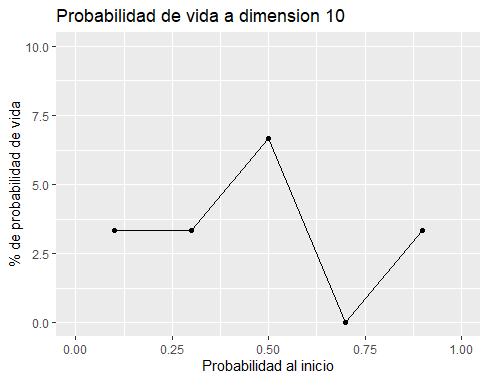
\includegraphics[width=100mm]{Figura1.png} % archivo
    \caption{Grafica que se obtiene a partir de la tabla \ref{Tab:Tabla2}}
    \label{Figura1}
\end{figure}

Los valores de la tabla \ref{Tab:Tabla2} se ven reflejados en la figura \ref{Figura1}  y se puede observar como la región central destaca muy poco por encima de las otras. la baja probabilidad se debe a la pequeña dimension con la que se trabajo. Se realizó el experimento varias veces más para revisar resultados y se obtuvo como máximo un 10\% de probabilidad de vida en diferentes probabilidades de vidas iniciales significando esto un máximo de 3 vidas creadas. 

\begin{figure} [h!]% figura
    \centering
    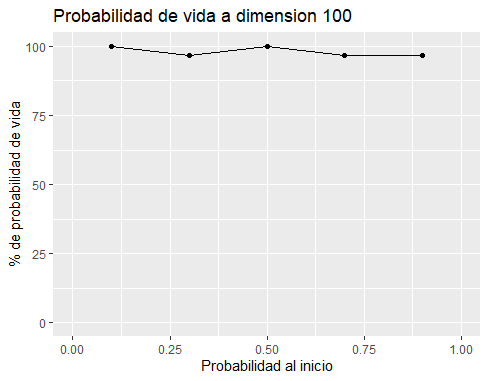
\includegraphics[width=100mm]{Figura2.png} % archivo
    \caption{Experimento realizado a dimensiones muy grandes}
    \label{Figura2}
\end{figure}

La figura \ref{Figura2} nos muestra un ejemplo de los resultados obtenidos para dimensiones grandes, en él se puede observar que la probabilidad de vida se obtiene de casi un 100 \% en todas las probabilidades iniciales debido a que hay más espacio para que esta se genere.

\section{Conclusiones}
En esta práctica aprendimos a agregar en cuenta la importancia de estados pasados para la generación de nuevos estados a partir de ciertas probabilidades dadas. A la vez que las interacciones entre vecinos tienen un efecto sobre los resultados obtenidos. La dimensión es un factor grande que determina la probabilidad de vida final independientemente de la inicial ya que a mayor dimensión mayor probabilidad de vida hay. La razón de que se obtuvieran graficas relativamente diferentes para cada experimento dentro del mismo rango de dimensión se puede deber a que son probabilidades iniciales y aunque con menor frecuencia, pueden llegar a los mismos valores de poder generar vida dentro del experimento. En lo personal me siento muy contento con el resultado ya que se trabajó exhaustivamente para la realización del presente trabajo.

\bibliography{referencias}
\bibliographystyle{plainnat}

\end{document}
